\documentclass{article}

\usepackage{tikz}

\begin{document}

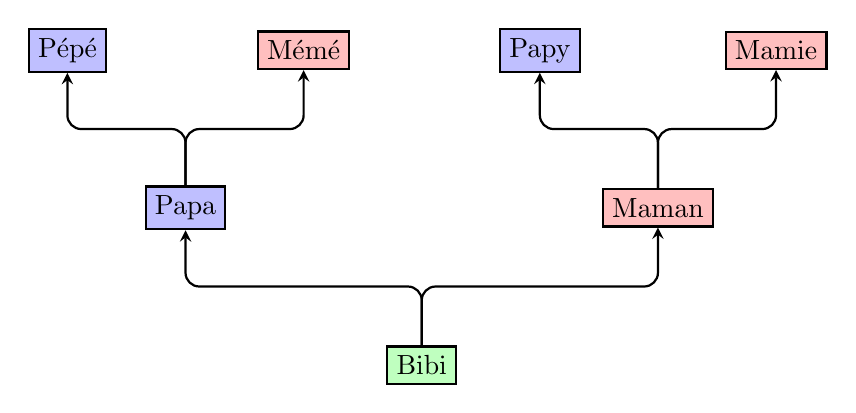
\begin{tikzpicture}
	\tikzstyle{lien}=[->,>=stealth,rounded corners=5pt,thick]
	\tikzset{individu/.style={draw,thick,fill=#1!25},
	         individu/.default={green}}
	\node[individu] (B) at (0,0) {Bibi};
	\node[individu=blue] (P) at (-3,2) {Papa};
	\node[individu=red] (M) at (3,2) {Maman};
	\node[individu=blue] (GPP) at (-4.5,4) {P\'ep\'e};
	\node[individu=red] (GMP) at (-1.5,4) {M\'em\'e};
	\node[individu=blue] (GPM) at (1.5,4) {Papy};
	\node[individu=red] (GMM) at (4.5,4) {Mamie};
	\draw[lien] (B) |- (-1,1) -| (P);
	\draw[lien] (B) |- (1,1) -| (M);
	\draw[lien] (P) |- (-4,3) -| (GPP);
	\draw[lien] (P) |- (-2,3) -| (GMP);
	\draw[lien] (M) |- (2,3) -| (GPM);
	\draw[lien] (M) |- (4,3) -| (GMM);
\end{tikzpicture}

\end{document}
